% DOCUMENT FORMATING
\documentclass[12pt]{article}
\usepackage[margin=1in]{geometry}

% PACKAGES
\usepackage{amsmath} % For extended formatting
\usepackage{amssymb} % For math symbols
\usepackage{amsthm} % For proof environment
\usepackage{array} % For tables
\usepackage{enumerate} % For lists
\usepackage{extramarks} % For headers and footers
\usepackage{fancyhdr} % For custom headers
\usepackage{graphicx} % For inserting images
\usepackage{multicol} % For multiple columns
\usepackage{verbatim} % For displaying code
\usepackage{tkz-euclide}
\usepackage{pgfplots}
\usepackage{mathtools}


% SET UP HEADER AND FOOTER
\pagestyle{fancy}
\lhead{\MyCourse} % Top left header
%\chead{\MyTopicTitle} % Top center header
\rhead{\MyAssignment} % Top right header
%\lfoot{\MyCampus} % Bottom left footer
\cfoot{} % Bottom center footer
%\rfoot{\MySemester} % Bottom right footer
\renewcommand\headrulewidth{0.4pt} % Size of the header rule
\renewcommand\footrulewidth{0.4pt} % Size of the footer rule
\newcommand{\ds}{\displaystyle}



% ----------
% TITLES AND NAMES 
% ----------

\newcommand{\MyCourse}{Math 241}
\newcommand{\MyAssignment}{Practice Midterm 1}
%\newcommand{\MySemester}{Spring 2020}
%\newcommand{\MyCampus}{University of Hawaii at Manoa}

% ----------
% BEGIN DOCUMENT
% ----------

\begin{document} 

\begin{enumerate}

\item The table below shows values of $f(x)$ and $g(x)$ for values of $x$. 

\begin{table}[h!]
    \centering
    \begin{tabular}{|c|c|c|}
        \hline
        \( x \) & \( f(x) \) & \( g(x) \) \\
        \hline
        0 & 1 & 4 \\
        1 & 2 & 0 \\
        2 & 3 & 1 \\
        3 & 4 & 2 \\
        4 & 0 & 3 \\
        \hline
    \end{tabular}
\end{table}
Find the following values
\begin{enumerate}
\item $(f\circ f)(2)$\\
\vfill
\item $(f\circ f\circ f)(4)$
\vfill
\item $(f\circ g)(3)$
\vfill
\item $(f\circ g\circ f)(0)$
\vfill
\end{enumerate}

\pagebreak

\item Below are the graphs of $f(x)$ and $g(x)$ both of whose domains are $[-2,2]$. Answer the following if they exist. Otherwise state why they do not.

\begin{center}
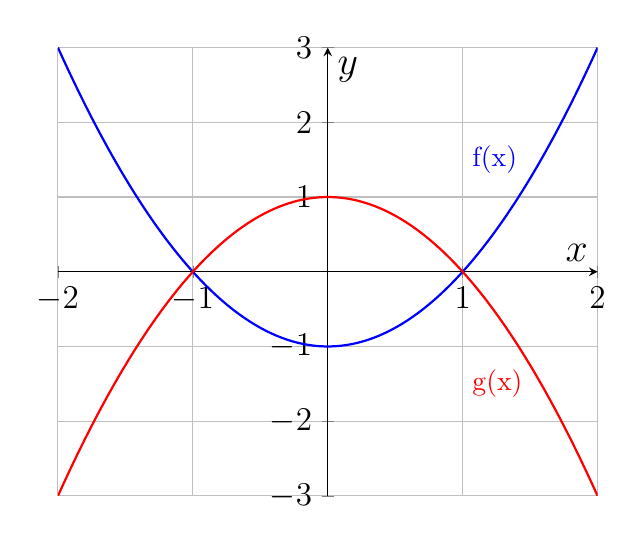
\begin{tikzpicture}
    \begin{axis}[
        axis lines=middle,
        xlabel={$x$},
        ylabel={$y$},
        xmin=-2, xmax=2,
        ymin=-3, ymax=3,
        xtick={-2,-1,0,1,2},
        ytick={-3,-2,-1,0,1,2,3},
        grid=major,
        every axis label/.append style={font=\Large},
        tick label style={font=\large},
    ]
        \addplot[domain=-2:2, samples=100, blue, thick] {x^2 - 1};
        \node[blue] at (axis cs:1,1.5) [right] {f(x)};
        
        \addplot[domain=-2:2, samples=100, red, thick] {-x^2 + 1};
        \node[red] at (axis cs:1,-1.5) [right] {g(x)};
    \end{axis}
\end{tikzpicture}    
\end{center}


\begin{enumerate}
    \item $(f\circ f)(0)$
    \vfill
    \item $(f\circ f)(2)$
    \vfill
    \item $(f\circ g)(0)$
    \vfill
    \item $(g\circ f)(1)$
    \vfill
\end{enumerate}
\pagebreak

\item Let $f(x) = x^2 + 4x + 6$ and let $g(x) = x^2 + 4$. What transformation takes $g(x)$ to $f(x)$? In other words, rewrite $f(x)$ as a function of $g(x)$ (in flip-shift) form and state what the transformation(s). \emph{Hint:} Complete the square on $f(x)$.

\pagebreak

\item Compute the following limits. If the limit is $\pm\infty$, state which. If the limit does not exist, write DNE. 

    \begin{enumerate}
        \item $\ds\lim_{x\to 1} \dfrac{x^3-2x^2+x}{x^2-1}$
        \vfill
        
        \item $\ds\lim_{x\to 0} \dfrac{\sqrt{x+16}-4}{x}$
        \vfill
        
        \item $\ds\lim_{x\to 0} \dfrac{\tan(3x)}{\tan(\pi x)}$
        \vfill
    
    
     \pagebreak
     
        \item $\ds\lim_{x\to 4} \sqrt{x^2-16}$
        \vfill

        \item $\ds\lim_{x\to -3^+} \dfrac{|x-3|-5}{2x+6}$
        \vfill

        \item $\ds\lim_{x\to 2} \dfrac{2x+1}{x^2-4}$
        \vfill
\end{enumerate}

\pagebreak
\item Below is the piecewise function $f(x)$.
\begin{comment}
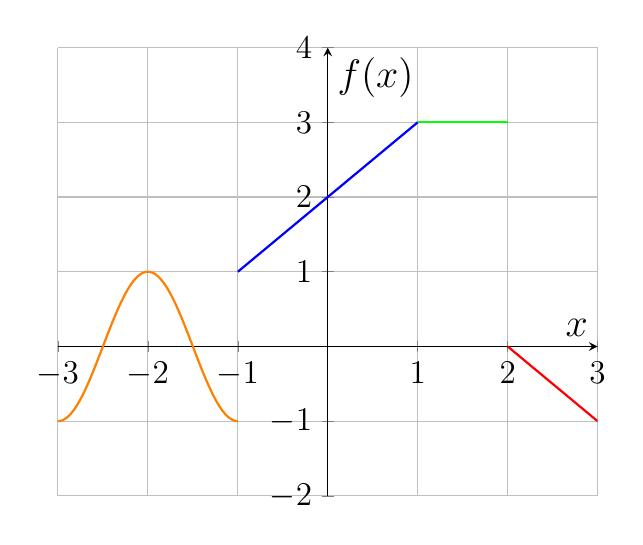
\begin{tikzpicture}
    \begin{axis}[
        axis lines=middle,
        xlabel={$x$},
        ylabel={$f(x)$},
        xmin=-3, xmax=3,
        ymin=-2, ymax=4,
        xtick={-3,-2,-1,0,1,2,3},
        ytick={-2,-1,0,1,2,3,4},
        grid=major,
        every axis label/.append style={font=\Large},
        tick label style={font=\large},
    ]
        % Cosine function for -3 <= x < -1
        \addplot[domain=-3:-1, samples=100, orange, thick] {cos(deg(pi*x))};
        
        % Linear function 1: x + 1 for -1 <= x < 1
        \addplot[domain=-1:1, samples=100, blue, thick] {x + 2};
        
        % Constant function: 3 for 1 <= x < 2
        \addplot[domain=1:2, samples=2, green, thick] {3};
        
        % Linear function: -x + 2 for 2 <= x <= 3
        \addplot[domain=2:3, samples=100, red, thick] {-x + 2};

    \end{axis}
\end{tikzpicture}
\end{comment}
$$f(x) = \begin{cases} \cos(\pi x)& -3 \leq x< -1\\
x+2& -1 \leq x < 1 \\ 3& 1\leq x < 2\\ -x+2& x\geq 2\end{cases}.$$

\begin{enumerate}
    \item Sketch the graph of $f(x)$.
    
    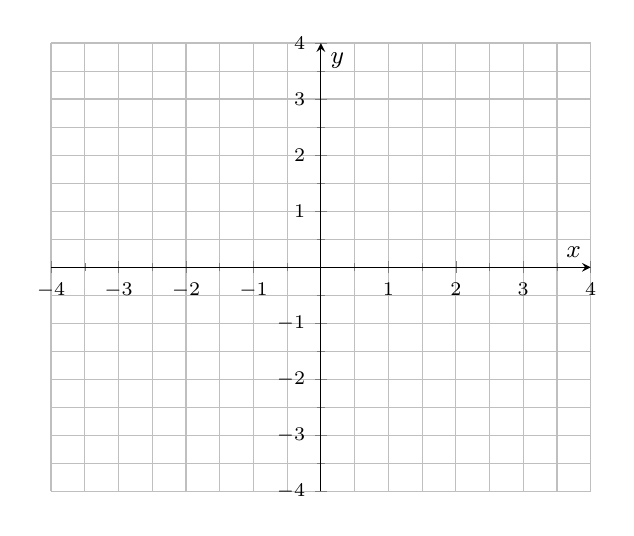
\begin{tikzpicture}
    \begin{axis}[
        axis lines=middle,
        xlabel={$x$},
        ylabel={$y$},
        xmin=-4, xmax=4,
        ymin=-4, ymax=4,
        xtick={-4,-3,...,4},
        ytick={-4,-3,...,4},
        grid=both,
        minor tick num=1,
        major grid style={line width=.5pt,draw=gray!50},
        %minor grid style={line width=.5pt,draw=gray!20},
        every axis label/.style={font=\small},
        tick label style={font=\scriptsize},
    ]
    \end{axis}
\end{tikzpicture}

\item Find the values of $a$ where $\ds\lim_{x\to a} f(x)$ does not exist.
\vfill

\item Find the values of $a$ where the function is discontinuous.
\vfill
\item Find the values of $a$ where $f$ is differentiable, but not continuous.
\vfill
\end{enumerate}

\pagebreak


\item The graph of a function $f$ is given below. Assume $f$ has vertical asymptotes at $x=-1$ and $x=1$.
	\begin{center}
	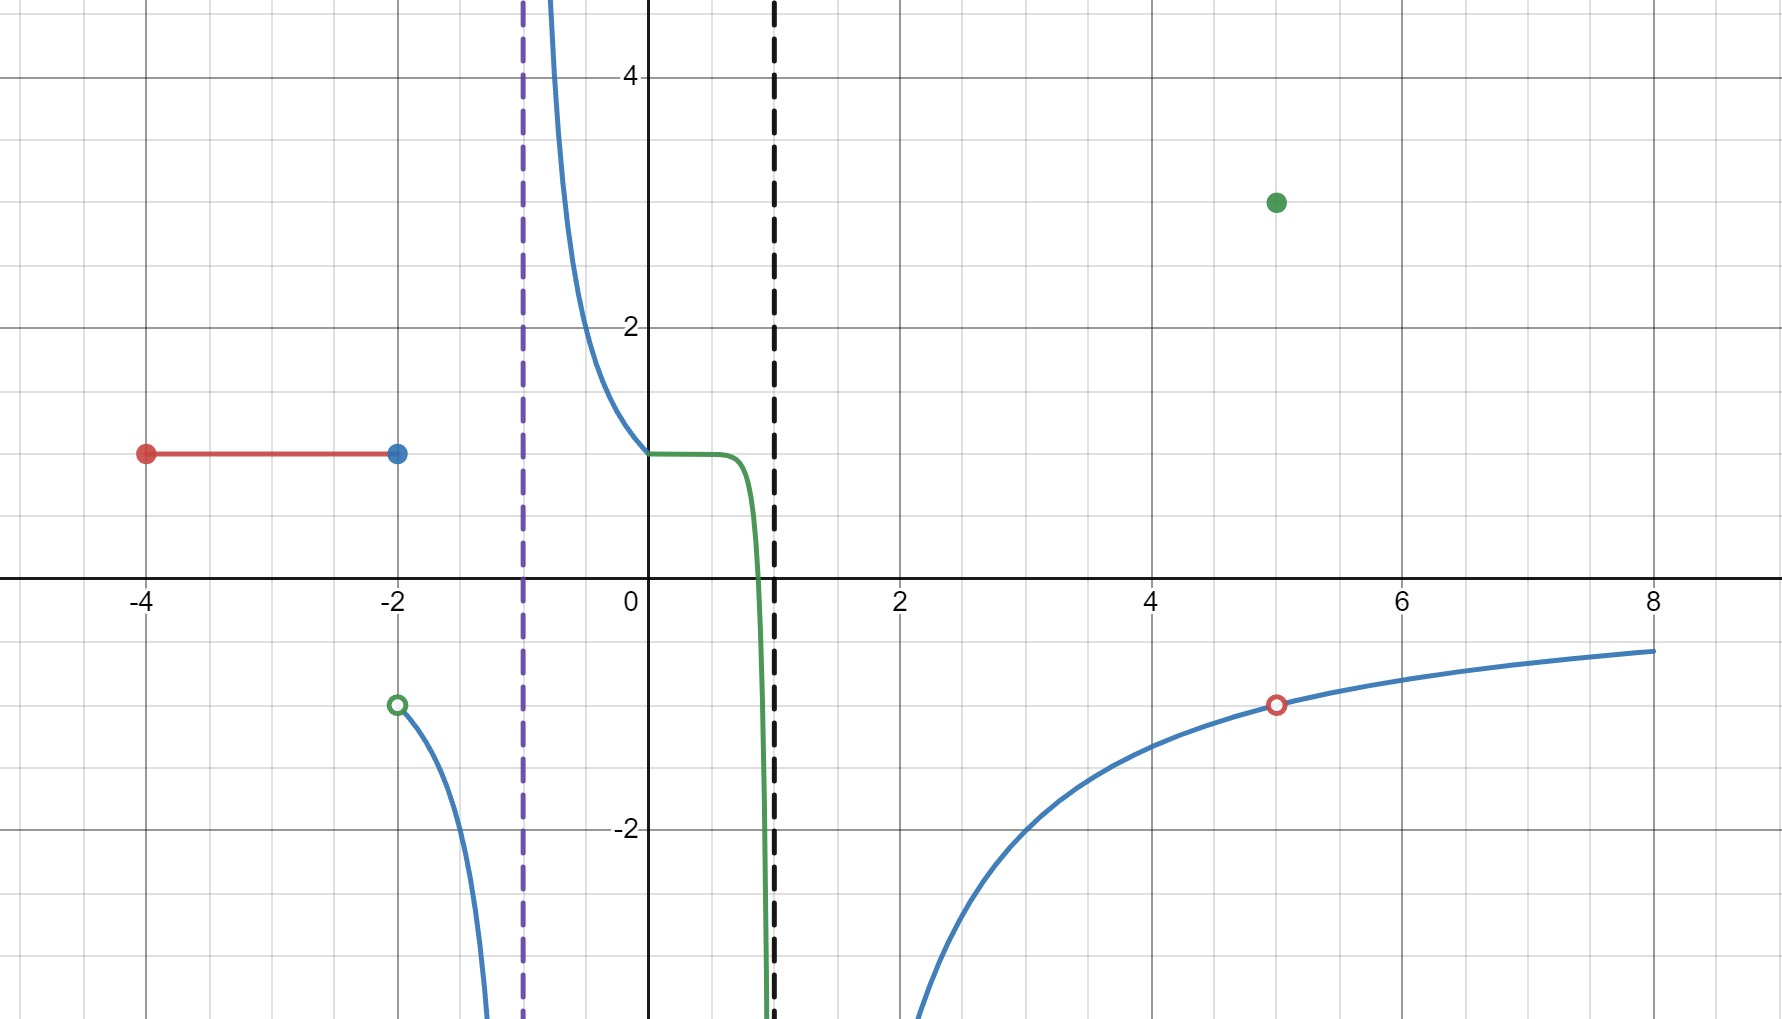
\includegraphics[width = 0.7\textwidth]{Images/S24M241_PMT1_pic1.jpeg}
	\end{center}
	\begin{enumerate}
		\item  Evaluate each of the following limits, or say the limit does not exist. If the limit is either $\infty$ or $-\infty$, specify which (rather than just say `does not exist').
		\begin{enumerate}
			\begin{multicols}{2}
				\item $\displaystyle\lim_{x\to 5} f(x)$\\
				\item $\displaystyle\lim_{x\to 1^-} f(x)$\\
				\item $\displaystyle\lim_{x\to 1^+} f(x)$ \\
                    \item $\displaystyle\lim_{x\to 1} f(x)$\\
				\columnbreak
				\item $\displaystyle\lim_{x\to -2^-} f(x)$\\ 
				\item $\displaystyle\lim_{x\to -2^+} f(x)$ \\
				\item $\displaystyle\lim_{x\to -2} f(x)$ \\
                    \item $\displaystyle\lim_{x\to 0} f(x)$ \\
			\end{multicols}
		\end{enumerate}
		
		\item  For which (if any) values in the interval $[-4,8]$ is the function $f$ not continuous?
		\vfill
		
		\item  For which (if any) values in the interval $[-4,8]$ is $f$ differentiable but not continuous?
		\vfill
		
		\item For which (if any) values in the interval $[-4,8]$ is $f$ continuous but not differentiable?
		\vfill
	\end{enumerate}
\pagebreak


 \item Find the derivative of the following functions.

 \begin{enumerate}
    \item $y(x) = \dfrac{4x^3 - 2\sqrt{x} + \frac{1}{x^7}}{x^2}$
    \vfill
    \item $z(s) = \dfrac{s^4 + 5s + 1}{s^3-4}$
    \vfill
    \item $w(t) = (t^2 - 8t)(t^{1/3} + 3)$
    \vfill

    \pagebreak

    \item $f(t) = \cos^2(\sqrt{t})$
    \vfill
    \item $g(s) = (10s^2 + 2s + 1)^{100}$
    \vfill
    \item $h(t) = \dfrac{t^2 + 4t}{1+\cos(t)}$
    \vfill
 \end{enumerate}

\pagebreak

\item  We are going to use  the \textbf{definition} of the derivative to compute $f'(t)$ for $f(t) = \dfrac{1}{t+1}.$

\begin{enumerate}
\item Using the definition of the derivative, write what $f'(t)$ is explicitly as a limit, but \textbf{do not simplify.}
\vspace{1in}
\item Find $f'(t)$ using your answer from part (a) above.
\vfill
\item Using the previous part, find the equation of the tangent line at $(3,\frac{1}{4})$.
\vspace{1in}
\end{enumerate}
\clearpage

\item  We are going to use  the \textbf{definition} of the derivative to compute $f'(1)$ for $$f(t) = \sqrt{x+8}.$$

\begin{enumerate}
\item Using the definition of the derivative, write what $f'(1)$ is explicitly, but \textbf{do not simplify.}
\vspace{1in}
\item Find $f'(1)$ by computing your answer from part (b) above.
\vfill
\end{enumerate}
\clearpage

\item Use implicit differentiation to find $\frac{dy}{dx}$ for $$x^3 + 4x^2y + y^2 = 8$$ at the point $(2,0)$ and find the equation of the tangent line at this point.
\clearpage

\item A particle moves with position function $$s = t^4-4t^3-20t^2+20t, \quad t\geq 0$$
where $s$ is in meters and $t$ is in seconds.
\begin{enumerate}
\item What is the velocity function?
\vspace{1in}
\item What is the acceleration function?
\vspace{1in}
\item At what time does the particle have a velocity of 20 m/s?
\vspace{2in}
\item At what time is the acceleration 0? 
\end{enumerate}

\pagebreak

\item A particle is moving along the curve $y = x^2$. As it reaches the point $(2,4)$, the $x$-coordinate is increasing at a rate of 2 cm/s. How fast is the distance from the particle to the origin changing at this instant?

\pagebreak
\end{enumerate}
\end{document}